\documentclass[]{beamer}
\usepackage{tikz}
%\usepackage[]{}
\author{Rémy \textsc{Taymans} \and Christophe \textsc{Degrelle}}
\title{Mutli-Agent Intersection Network}
\institute{ECAM} 
\date{\today} 


\AtBeginSection[]
{
  \begin{frame}
    \tableofcontents[currentsection,hideothersubsections, 
          sectionstyle=show/shaded]
  \end{frame}
}

\addtobeamertemplate{navigation symbols}{}{%
    \usebeamerfont{footline}%
    \usebeamercolor[fg]{footline}%
    \hspace{1em}%
    \insertframenumber/\inserttotalframenumber
}
    
\begin{document}
\begin{frame}
  \titlepage
\end{frame}


\begin{frame}{Table of Contents}
  \tableofcontents
\end{frame}


\section{Context}
\begin{frame}{Context}
\begin{block}{Reference article}
\centering
\emph{Schedule-Driven Coordination for Real-Time Traffic Network Control}
\end{block}

% from Xiao-Feng Xie, Stephen F. Smith and Gregory J. Barlow - 2012

 \begin{itemize}
  \item Real-time optimization of vehicle traffic
  \item Network of signalized intersections
  \item One intersection = one agent
  \item Prediction of traffic
  \item Optimizes movement of the observable traffic
 \end{itemize}
\end{frame}


\begin{frame}{Article Parameters}
 \begin{columns}
  \begin{column}[c]{5cm}
   \begin{itemize}
    \item Test multiple decision \textbf{algorithms}
    \item Send \textbf{cluster} between intersection
    \item Give the \textbf{time} and the \textbf{density} of traffic
   \end{itemize}
  \end{column}

  \begin{column}[c]{5cm}
   \begin{figure}
    \centering
    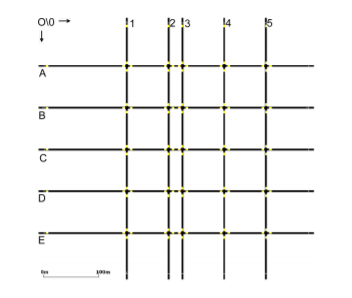
\includegraphics[width=\textwidth]{img/grid.png}
   \end{figure}
  \end{column}
 \end{columns}
 $Cluster = (density, arrival, departure)$
\end{frame}


\section{Objective}
\begin{frame}{Objective}
 \begin{itemize}
  \item Simulate an intersection
  \item Analyze different algorithms
  \item Allow information propagation between intersection
  \item Decrease the cumulative delay
 \end{itemize}
\end{frame}


\begin{frame}{Which approach to use ?}
 \begin{block}{No software available in the article}
 $\rightarrow$ Simulate a little part of the network and observe the performances of different algorithms
 \end{block}
 
 \begin{block}{Questions}
  \begin{itemize}
   \item Which parameters do we need ?
   \item Where do we get information ?
   \item Which size of grid ?
  \end{itemize} 
 \end{block}
\end{frame}


\section{Simplifications}
\begin{frame}{The agent}

 \begin{columns}
  \begin{column}[c]{4cm}
  Simplifications
   \begin{itemize}
    \item Two ways
    \item One intersection
    \item No turns allowed
   \end{itemize}
   Parameters
   \begin{itemize}
    \item Yellow duration
    \item Startup lost time
   \end{itemize}
  \end{column}
  \begin{column}[c]{6cm}
   \begin{figure}
    \begin{tikzpicture}[thick,scale=0.75, every node/.style={scale=0.75}]
     \draw[->, line width = 1.5] (0,0) -- (5,0);
     \draw[->, line width = 1.5] (2.5,2.5) -- (2.5,-2.5);
     \node at (2.5,0) {\textbullet};

     \node at (0,0) [left] {Input 1};
     \node at (2.5,2.5) [above] {Input 2};
     \node at (2.5,-2.5) [below] {Output 2};
     \node at (5,0) [right] {Output 1};
    \end{tikzpicture}
   \end{figure}
  \end{column}
 \end{columns}
 \vspace{1cm}
 
 \centering
 $Cluster = (vehicules, arrival, departure, waiting\_time)$
\end{frame}


\section{Algorithms}
\begin{frame}{First Test : Fixed Time Intersection}
 \begin{itemize}
  \item Opening time fixed for each ways
  \item Same behaviour whatever inputs
 \end{itemize}
 \begin{block}{Conclusion}
  $\rightarrow$ Not cooperative\\
  $\rightarrow$ Basic vision of current intersections
 \end{block}
\end{frame}


\begin{frame}{Second Test : FCFS without Prehension Intersection}
 \begin{itemize}
  \item First came first served
  \item Do not cut a cluster
 \end{itemize}
 \begin{block}{Conclusion}
  $\rightarrow$ Able to cooperate\\
  $\rightarrow$ Find only local but not global optimum
 \end{block}
\end{frame}


\section{Perspectives}
\begin{frame}{Perpectives}
Implement grid with several agents\vspace{0.5cm}

Test other algorithms :
 \begin{itemize}
  \item FCFS with prehension
  \item Manage priorities in function of the total waiting time, the length of cluster, the prior vehicules,...
 \end{itemize}
 \vspace{0.5cm}
 Consider the global impact of the choices in the network, not only the local one
\end{frame}


\begin{frame}
\centering \LARGE
  \emph{Any questions ?}
\end{frame}


\begin{frame}{References}
%Name, Year, \emph{title}, \url{}
XF Xie, SF Smith, GJ Barlow, 2012, \emph{Schedule-Driven Coordination for Real-Time Traffic Network Control}.
\end{frame}
\end{document}
